%\documentclass[12pt]{book}
%\usepackage[width=5.5in,height=8.5in,
%  hmarginratio=3:2,vmarginratio=1:1]{geometry}
%
%% for some of these packages, you might have to install
%% texlive-latex-extra (in Ubuntu)
%
%\usepackage[T1]{fontenc}
%\usepackage{textcomp}
%\usepackage{mathpazo}
%\usepackage{pgfplots}
%%\pgfplotsset{compat=newest}
%%\usepackage{pslatex}
%
%\usepackage{url}
%\usepackage{fancyhdr}
%\usepackage{graphicx}
%\usepackage{subfig}
%\usepackage{amsmath}
%\usepackage{amsthm}
%%\usepackage{amssymb}
%\usepackage{makeidx}
%\usepackage{setspace}
%\usepackage{hevea}                           
%\usepackage{upquote}
%
%
%% these styles get translated in CSS for the HTML version
%\newstyle{a:link}{color:black;}
%\newstyle{p+p}{margin-top:1em;margin-bottom:1em}
%\newstyle{img}{border:0px}
%
%% change the arrows in the HTML version
%
%\makeindex
%
%
%\begin{document}


%
%
%\newcount\anchorcnt
%\newcommand*{\Anchor}[1]{%
%  \@bsphack%
%    \Hy@GlobalStepCount\anchorcnt%
%    \edef\@currentHref{anchor.\the\anchorcnt}% 
%    \Hy@raisedlink{\hyper@anchorstart{\@currentHref}\hyper@anchorend}% 
%    \M@gettitle{}\label{#1}% 
%    \@esphack%
%}
%
%
%
%%%% EXERCISE
%
%\newtheoremstyle{exercise}% name of the style to be used
%  {\topsep}% measure of space to leave above the theorem. E.g.: 3pt
%  {\topsep}% measure of space to leave below the theorem. E.g.: 3pt
%  {}% name of font to use in the body of the theorem
%  {0pt}% measure of space to indent
%  {\bfseries}% name of head font
%  {}% punctuation between head and body
%  { }% space after theorem head; " " = normal interword space
%  {}% Manually specify head
%
%\theoremstyle{exercise}
%\newtheorem{exercise}{Exercise}[chapter]
%
%%\newcounter{exercise}[chapter]
%%\newcommand{\nextexercise}{\refstepcounter{exercise}}
%
%%\newenvironment{exercise}{\nextexercise  \textbf{Exercise \thechapter.\theexercise} \begin{itshape} }{\end{itshape}}
%
%%\blankpage
%
%
%

\chapter{Descriptive statistics}
\label{descriptive}
\section{Significance}

Experiments are at the heart of the field of physics. The theories, laws and models relies on observations and experimentations. The gathering of data and analysis is an intrinsic part of physics. However, how do we go about turning data into theories, laws and models? Statistics is our friend  and in this chapter we will introduce a few notions about the analysis and interpretation of data. 

Say you want to determine the time of fall of steel balls in a cylinder filled with water over a distance of one meter.  You replicate the measurement several times  and collect your data into a table. One of your friend perform a similar experiment with a narrower cylinder. You find that on average the time of fall is slower by 2 ms in the narrow cylinder. 

\index{apparent effect}

A difference like that is called an {\bf apparent effect}; that is,
there might be something going on, but we are not yet sure.  There are
several questions we still want to ask:

\begin{itemize}

\item If the two experiments have different means, what about other {\bf
  summary statistics}, like median and variance?  Can we be more
  precise about how they differ?
\index{summary statistic}

\item Is it possible that the difference we saw could occur by chance,
  even if the experiments we compared were actually the same?  If so,
  we would conclude that the effect was not {\bf statistically
    significant}.
\index{statistically significant}
\index{significance}


\item Is it possible that the apparent effect is due to selection bias or
  some other error in the experimental setup?  If so, then we might
  conclude that the effect is an {\bf artifact}; that is, something we
  created (by accident) rather than found. 
\index{artifact}

\end{itemize}

Answering these questions will take most of the rest of this chapter.

\section{Errors}
 Before we go into details of error analysis it is important to understand the meaning of error in science. Error in a scientific measurement usually does not mean a mistake or blunder. Instead, the terms ``error'' and ``uncertainty'' both refer to unavoidable imprecision in measurements.

Of course, not all measurements have errors. If asked how many people there are in a room, one can usually give an exact number as an answer. However, if we want to know how many atoms there are in a room, giving an exact answer is nearly impossible, as the animation below illustrates.

In the physical science, you will deal mostly with measurements of the second kind. Since you will not be able to measure things with arbitrarily high precision, you should know how to quantify the imprecision of your results.
 Under different circumstances, the error that we are off by may vary greatly, so it is very useful to have a measurement of the quality of the measurement, which we call the {\bf error analysis}. First we choose a physical {\bf quantity} $X$ to determine and then we perform an {\bf experiment} which is a set of measurements of this quantity. Each {\bf measurement} gives a {\bf value} $x_i$. The {\bf outcome} $O_X$ of the experiment is the set of all results. Finally, we present the {\bf result} $\bar{x}$, which is the mean of the results in the outcome. The {\bf true value} $X_o$ is the value that would be measured if our experiment had no error. A good experiment will produce a result very close to the true value, $\bar{x} \cong X_o$.

Sources of error are commonly classified as either {\it systematic error} or {\it random error}. A {\bf systematic error} is any error that skews the measured values by the same amount in the same direction every time.\footnote{If an error source skews the measured values by a roughly constant amount in one direction, but has a slightly different effect each time, then it is probably an error source that has both a systematic and a random component.} For example, if you were making measurements with a stopwatch that always started at 0.01s instead of 0.00s, then you would have a systematic error. A {\bf random error} is any error that is not a systematic error. For example, if you were measuring an object with a ruler and you were off by a fraction of a millimeter, then you would have a random error. 

Random error usually skews measured values higher and lower with equal probability. If this is the case, then it possible to eliminate it by averaging, which we will denote averaging by enclosing the expression in angle brackets or covering it with a bar. First, we represent the value of a measurement by breaking it down into three components.

\[\textrm{Measurement = True Value + Systematic Error + Random Error}\]

%When we take the average of the measurements, we mean the exact average, which would be the average that you would obtain if you made the measurement an infinite number of times and averaged your results. 
Now averaging is distributive so we have

\[\langle \textrm{Measurement} \rangle  = \langle\textrm{True Value}\rangle + \langle\textrm{Systematic Error}\rangle + \langle\textrm{Random Error}\rangle \]

The first two terms on the right hand side are just constants, so we can drop the averaging symbols on them. The last term has an average of approximately zero in most cases yielding

\[\langle \textrm{Measurement} \rangle \textrm{ = True Value + Systematic Error}\]

We can't get rid of the systematic error with statistical methods, but by using quality equipment and improving our experimental technique we can usually reduce systematic error to a negligible level. Therefore, if you average your measured values and take care to minimize systematic error then you will obtain a result that is approximately equal to the true value.

It is not always the case that random error cancels with averaging. For example, if you are measuring the speed of a rolling ball and there is an intermittent breeze that is always in the same direction, then there will be a random error in the speed that biases it in one direction. Averaging will not be able to eliminate this type of random error. 

The most common measurements in the lab are done with devices that have a marked scale. There in an intrinsic limitation to the precision of our measurement. Say me measure the length of a pendulum. We find that is certainly closer to 128.9 cm than to 128.8 cm or 129.0 cm. Thus we can state with absolute confidence that the length is 128.8cm $\pm$ 0.1 cm. We call the first term, 128.9 cm, the "central value" and the second term, 0.1 cm, the "error" or "uncertainty" \footnote{We will revisit this subject later on.  Suffice to say this is a worst-case scenario. Most likely the error is much smaller. We will see later on that the standard uncertainty is given $\frac{(129.0-128.8)}{2\sqrt{6}}=0.04$~cm.}.

Many modern laboratory instruments use digital displays. For example, you can measure weights using an electronic scale. It has the advantage that you don't have to judge what is the central value of your measurement. It will give you the central value. All you have to do is write it down. Now, what is the error of this seemingly "precise" measurement? All instruments, no matter how sophisticated, have a limit to their precision. Usually, the manufacturer of the instrument will specify the error. (Most of the time it is written on the back of the instrument.) However, if you can't find this information, use the following rule of thumb: The error of an electronic device is usually half of the last precision digit. The following example should make it clear. Suppose you measured your weight with the electronic device pictured above. The result is 138.2 lbs. What is the error? If you can't find the manufacturer information about the error, you notice that the resolution of your measurement is 0.1 lb. In other words, the device claims that it can give you a more precise value than 138 lbs, but it doesn't tell you whether your weight is 138.15 lbs or 138.25 lbs. Thus we can assume that the error of our measurement is 0.05 lb. And our answer is 138.2 lbs $\pm$ 0.05 lb \footnote{Again this is an upper bound to the error,  the standard uncertainty is $\frac{(138.25-138.15)}{2\sqrt{3}}=0.03$~lb.}.

Not all measurements are done with instruments whose error can be reliably estimated. A classic example is the measuring of time intervals using a stopwatch. Of course, there will be a read-off error as discussed in the previous sections. However, that error will be negligible compared to the dominant error, the one coming from the fact that we, human beings, serve as the main measuring device in this case. Our individual reaction time in starting and stopping the watch will be by far the major source of imprecision. Since humans don't have built-in digital displays or markings, how do we estimate this dominant error?

The solution to this problem is to repeat the measurement many times. Then the average of our results is likely to be closer to the true value than a single measurement would be. 

\section{Means and averages}
\label{mean}

If you have a sample of $N$~values, $x_i$, the mean, $\bar{x}$, is
the sum of the values divided by the number of values; in other words
%
\[ \bar{x} = \frac{1}{N} \sum_{i=1}^N x_i \]
%

Another standard notation for the average is $\langle x\rangle$.

Now, suppose you measure the oscillation period of a pendulum with a stopwatch five times. You obtain the following data (in seconds):
\begin{verbatim}
3.55, 3.65, 3.73, 3.59, 3.67
\end{verbatim}

We find the mean period of oscillations is :

\[ \bar{x} = \frac{3.55+ 3.65+ 3.73+3.59+3.67}{5} = 3.65 \text{s}\]

The words ``mean'' and ``average'' are sometimes used interchangeably,
but we will maintain this distinction:

\begin{itemize}

\item The ``mean'' of a sample is the summary statistic computed with
  the previous formula.

\item An ``average'' is one of many summary statistics you might
  choose to describe the typical value or the
  {\bf central tendency} of a sample.
\index{central tendency}

\end{itemize}

Sometimes the mean is a good description of a set of values.  For
example, apples are all pretty much the same size (at least the ones
sold in supermarkets).  So if I buy 6 apples and the total weight is 3
pounds, it would be a reasonable summary to say they are about a half
pound each.
\index{weight!pumpkin}

But pumpkins are more diverse.  Suppose I grow several varieties in my
garden, and one day I harvest three decorative pumpkins that are 1
pound each, two pie pumpkins that are 3 pounds each, and one Atlantic
Giant that weighs 591 pounds.  The mean of
this sample is 100 pounds, but if I told you ``The average pumpkin
in my garden is 100 pounds,'' that would be wrong, or at least
misleading.
\index{pumpkin}

In this example, there is no meaningful average because
there is no typical pumpkin.



\section{Distributions}
\label{distributions}
\index{distribution}

Summary statistics are concise, but dangerous, because they obscure
the data.  An alternative is to look at the {\bf distribution} of the
data, which describes how often each value appears.

The most common representation of a distribution is a {\bf histogram},
which is a graph that shows the frequency or probability
of each value.\index{histogram}. A {\bf histogram} is a chart made by stacking up squares in columns based on the values of measurements, with one square added per measurement. This makes the more frequent results form taller columns.

\begin{figure}[h]
\begin{center}
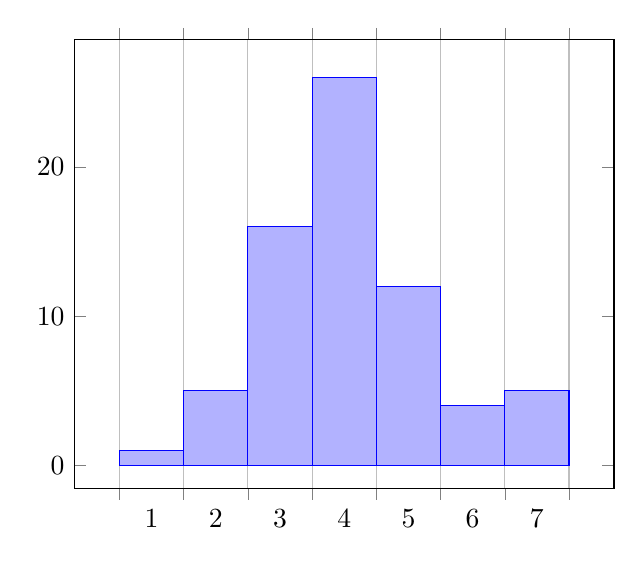
\begin{tikzpicture}
\begin{axis}[
ybar interval,
xtick={1,2,3,4,5,6,7,8},% reset from ybar interval
%xticklabel=
%{$[\pgfmathprintnumber\tick,%
%\pgfmathprintnumber\nexttick)$}
%]
]
% a data file containing 8000 normally distributed
% random numbers of mean 0 and variance 1

\addplot coordinates {
    (1,1) (2,5) (3,16)
     (4,26) (5,12) (6,4) (7,5) (8,2)};
\end{axis}
\end{tikzpicture}
\caption{Sample Histogram}
\end{center}
\end{figure}

In this figure, each square represents one measurement of a quantity $X$. The value of the measurement, which we call $x$, is the number of the column that it lies in. We can write the value of the $i^{th}$ measurement as $x_i$. Most quantities that we measure are not always integers, but we can still use histograms by making each column a {\bf bin} that collects any value falling within a specific range. We will refer to the shape that the histogram forms as a {\bf distribution} of measurements. 

There are two distinct measures of the error of a result, {\it accuracy} and {\it precision}. The {\bf accuracy} tells you how close your result is to the accepted result. Accuracy is almost always expressed in terms of the {\bf percent error}
\footnote{Percent error is also called percent deviation}, which is given by 
\begin{equation}\frac{\textrm{Experimental Result} - \textrm{Accepted Result}}{\textrm{Accepted Result}} \times 100 \end{equation}

The {\bf precision} tells you how consistent your measured values are, with higher precision indicating that all of your data points are clustered around one value. Effectively, precision is a measure of the width of the distribution for the experiment. In order to quantify the width of the distribution we need a formula that accounts for the contribution to the spread by each measured value. The first thing that comes to mind is the {\bf deviation} of each value, which is given by 
\begin{equation} d_i \equiv x_i - \bar{x} \end{equation}

but this won't help to much because if we average the deviation over all the values, we will usually get an answer close to zero. This is because random error usually is equally likely to skew the values in either direction from the average and this will cause the deviations to cancel positive with negative. But there is a quick fix for this---we can just take the absolute value of the deviation and average that. This defines the {\bf mean deviation} \footnote{The mean deviation is also called the average deviation}
\begin{equation} \alpha_{O_X} = \frac{1}{N} \sum_i |x_i - \bar{x}| \end{equation}
where the subscript $O_X$ indicates that the expression is computed using the outcome of the experiment measuring the quantity $X$.

The mean deviation is not used very often. Instead of taking the absolute value, the square of the deviation is used. The square is again always positive, but it is more convenient than the absolute values because squares are easier to work with analytically and there are other advantages that we will see soon. Averaging the square of the deviation gives us the {\bf variance} 
\footnote{This is the biased or population standard deviation. There are arguments that it is better to divide by N-1 instead of N in the average, but we will not pursue that here}
\begin{equation}\sigma^2_{O_X} = \frac{1}{N} \sum_{i=1}^N \left(x_i - \bar{x}\right)^2  \end{equation}
%
%There is a useful identity involving the standard deviation that can be derived easily.
%\[\sigma_{O_X}^2 = \left\langle (x_i - \langle x_i \rangle)^2 \right\rangle 
%= \left\langle x_i^2 - 2x_i\langle x_i \rangle + \langle x_i \rangle^2 \right\rangle \]
%\[ = \langle x_i^2 \rangle - \langle 2x_i\langle x_i \rangle \rangle + \langle x_i \rangle^2 \]
%\[ = \langle x_i^2 \rangle - 2\langle x_i \rangle^2 + \langle x_i \rangle^2 
% = \langle x_i^2 \rangle - \langle x_i \rangle^2\]

In the same way that the mean is intended to describe the central
tendency, variance is intended to describe the {\bf spread}.
The variance of a set of values is\footnote{You may have seen or learned another definition of the variance in which $N-1$ is replaced by $N$. Technically the variance must include the $N$ factor whereas the sample variance includes the $N-1$ factor. The sample variance is an ``unbias'' estimator of the variance. It's more of a mathematical subtlety, which does not affect our reasoning here. In any case, the difference between the two is negligible for large $N$. See
\url{http://wikipedia.org/wiki/Bias_of_an_estimator} for more information.
 }
%
\[ s^2 = \frac{1}{N-1} \sum_{i=1}^N \left(x_i - \bar{x}\right)^2 \]
%
The term $x_i-\bar{x}$~is called the ``deviation from the mean,'' so
variance is the mean squared deviation, which is why it is denoted $s^2$.  


 
The variance is our previous example is
\begin{align*}
 s^2 =\frac{1}{5-1} [&(3.55-3.65)^2+ (3.65-3.65)^2+ (3.73-3.65)^2\\
 &+(3.59-3.65)^2+(3.67-3.65)^2 ] = 0.0051  \text{s}^2
\end{align*}




The square root of variance, $s$, is called the {\bf
  standard deviation}.
\index{deviation}
\index{standard deviation}


By itself, variance is hard to interpret.  One problem is that the
units are strange; in this case the measurements are in pounds, so the
variance is in pounds squared.  Standard deviation is more meaningful;
in this case the units are pounds.



Now we want to consider the shape that a histogram of the outcome would take if we had performed an infinite number of measurements. This limiting distribution would give us a sense for what the error itself really looks like instead of just seeing a few pieces of the puzzle. Without further information about the measurement process, we can't be sure what the histogram would look like. But the {\bf central limit theorem} proves that if the measurement process is affected by many independent random errors, then the limiting distribution of an infinite number of measurements will be approximately a {\it Gaussian distribution}. Whether or not this is the reason, it is true that very often random error in measurements produces a {\bf Gaussian distribution}, which is a bell-shaped curve with the functional form
\begin{equation} f(x) = \frac{1}{\sigma \sqrt{2 \pi}}  e^{-\frac{(x-\mu)^2}{2\sigma^2}}\end{equation}
where $\sigma$ is the width parameter, and $\mu$ is the center of the peak. These parameters are just numbers to plug into the formula, but their symbols were chosen because $\sigma$ is the standard deviation of the limiting distribution and $\mu$ is the average of the limiting distribution.

\begin{figure}[h]
\begin{center}
\definecolor{qqqqff}{rgb}{0,0,1}
\definecolor{qqqqqq}{rgb}{1,0,0}
%\begin{tikzpicture}[line cap=round,line join=round,>=triangle 45,x=1.0cm,y=10.0cm]
\begin{tikzpicture}[line cap=round,line join=round,>=,x=1.0cm,y=10.0cm]
\draw[->,color=black] (-3.99623,0) -- (3.81526,0);
\draw[->,color=black] (-3.5,-0.08169) -- (-3.5,0.49561);
%\clip(-3.49623,-0.38169) rectangle (3.81526,0.69561);
\draw[color=qqqqff,fill=qqqqff,fill opacity=0.25, smooth,samples=50,domain=-1.00:1.00] plot(\x,{1/sqrt(2*3.1415926535)*exp(-0.5*(\x)^2)}) -- (1.0,0) -- (-1.0,0) -- cycle;
\draw[line width=2pt,color=qqqqqq, smooth,samples=100,domain=-3.4962341176758:3.81525635549043] plot(\x,{1/sqrt(2*3.1415926535)*exp(-0.5*(\x)^2)});
\draw [color=black](1.00,-0.02) node[anchor=north] {$\mu+\sigma$};
\draw [color=black](-1.00,-0.02) node[anchor=north] {$\mu-\sigma$};
\draw [color=yellow](-0.54691,0.1499) node[anchor=north west] {\textbf{Area}};
\draw [color=yellow](-0.54691,0.0999) node[anchor=north west] {\textbf{0.68}};
\draw[color=blue] (-4.2325,0.45082) node {$y$};
\draw[color=blue] (3.23,-0.0582) node {$x$};
\draw[color=blue] (-0.03,-0.0582) node {$\mu$};
\fill [color=black] (1.00,0) circle (1.5pt);
\fill [color=black] (-1.00,0) circle (1.5pt);
\end{tikzpicture}

\caption{Gaussian Distribution: $ f(x) = \frac{1}{\sigma \sqrt{2 \pi}}  e^{-\frac{(x-\mu)^2}{2\sigma^2}}$. The probability that the value $x$ ranges from $\mu -\sigma$  to $\mu +\sigma$ is 68\%.  }
\end{center}
\end{figure}

The gaussian distribution is an example of a probability density function (PDF). Evaluating a PDF for a particular value of $x$~is usually not useful.
The result is not a probability; it is a probability {\em density}.
\index{density}
\index{mass}

In physics, density is mass per unit of
volume; in order to get a mass, you have to multiply by volume or,
if the density is not constant, you have to integrate over volume.
\index{inertia}
\index{moment of inertia}

% Similarly, probability density measures probability per unit of $x$.
% In order to get a probability mass, you have to integrate over $x$.
% For example, if $x$~is a random variable whose PDF is PDF$_X$, we
% can compute the probability that a value from $x$~falls between 
% $-$0.5 and 0.5:

% \[ P(-0.5 \le X < 0.5) = \int_{-0.5}^{0.5} PDF_{X}(x) dx \]


In this context, {\bf frequency} means the number of times a value
appears in a dataset---it has nothing to do with the pitch of a sound
or tuning of a radio signal.  A {\bf probability} is a frequency expressed
as a fraction of the sample size, $N$.
\index{frequency}
\index{probability}
\index{dictionary}


The result is a dictionary that maps from values to frequencies.
To get from frequencies to probabilities, we divide through by $N$,
which is called {\bf normalization}:\index{normalization}

\begin{equation}
\text{Relative frequency} = \text{the number of readings in the bin}
\end{equation}

The normalized histogram is called a {\bf PF}, which stands for
``probability function''; that is, it's a function that maps from
values to probabilities.
\index{PF}
\index{probability function}

To illustrate the idea, suppose we measure the time of fall of the steel balls  as discussed in the previous section, until we have 12 measurements (in seconds):

2.3, 2.4, 2.5, 2.6, 2.5, 2.3, 2.4, 2.4, 2.2, 2.4, 2.5, 2.5

Histograms and probability functions are most often plotted as bar charts.  Figure~\ref{pendulum} shows a histogram of the oscillation period of pendulum. 

\begin{figure}[h]
\begin{center}
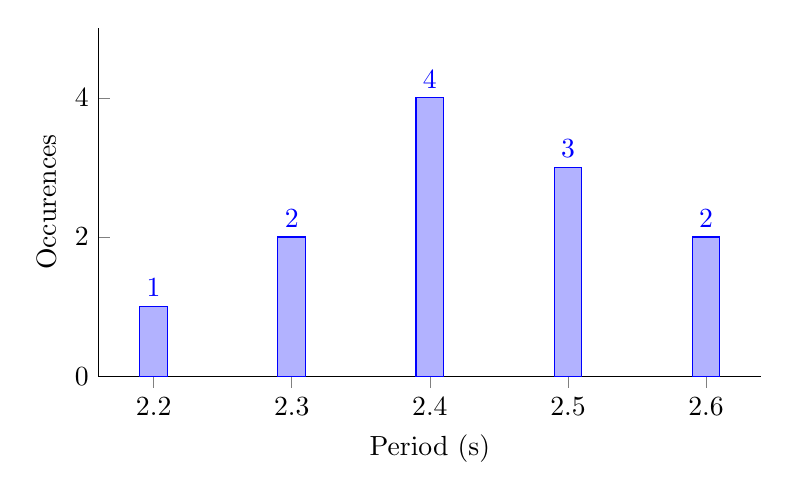
\begin{tikzpicture}
  \centering
  \begin{axis}[
        ybar,
    height=6cm,
    width=10cm,
    enlarge y limits=false,
    axis lines*=left,
    ymin=0,
    ymax=5,
     legend style={at={(0.5,-0.2)},
        anchor=north,legend columns=-1},
        ylabel={Occurences},
        xlabel={Period (s)},
     xtick=data,
        nodes near coords,
    ]
    \addplot coordinates {
    (2.2,1) (2.3,2) (2.4,4)
      (2.5,3) (2.6,2)};
  \end{axis}
\end{tikzpicture}
\end{center}
\caption{ \quad Histogram of the period of pendulum.}
\label{pendulum}
\end{figure}

Histograms are useful because they make the following features immediately
apparent:

\begin{description}

\item[Mode:] The most common value in a distribution is called the
  {\bf mode}.  In Figure~\ref{pendulum} there is a clear mode at 2.4 s.  In this case, the mode is the summary statistic that does
  the best job of describing the typical value.
\index{mode}

\item[Shape:] Around the mode, the distribution is asymmetric; it
  drops off quickly to the left and more slowly to the right.  In statistics this is often referred to as a skew. 
\index{shape}

\item[Outliers:] Values far from the mode are called {\bf outliers}.
  Many of them are probably due to errors, either in the reporting
  or recording of data.
\index{outlier}

\end{description}

Although histograms make some features apparent, they are usually not
useful for comparing two distributions.  We can address this problem using probability functions.


\section{Probability Functions (PF's)}
\index{plotting}
\index{PF}


To plot a probability function as a bar graph:  Bar graphs are most useful if the number
of values in the probability function is small.

\begin{figure}[h]
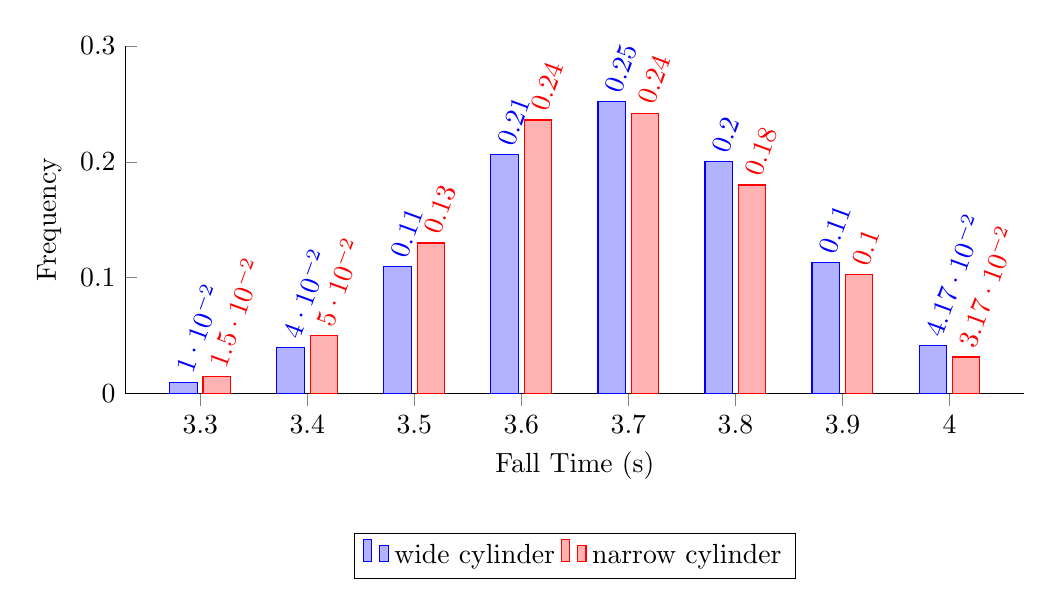
\begin{tikzpicture}
  \centering
  \begin{axis}[
        ybar,
    height=6cm,
    width=13cm,
    enlarge y limits=false,
    axis lines*=left,
    ymin=0,
    ymax=0.3,
     legend style={at={(0.5,-0.4)},
        anchor=north,legend columns=-1},
        ylabel={Frequency},
        xlabel={Fall Time (s)},
     xtick=data,
        nodes near coords,
    every node near coord/.append style={
        anchor=mid west,
        rotate=70
    }
    ]
    \addplot coordinates { (3.3, 0.01) (3.4, 0.04) (3.5, 0.11) (3.6, 0.206) (3.7, 0.252)(3.8, 0.20) (3.9, 0.113)  (4.0, 0.0417)  };
        \addplot coordinates { (3.3, 0.015) (3.4, 0.05) (3.5, 0.13) (3.6, 0.236) (3.7, 0.242)(3.8, 0.18) (3.9, 0.103)  (4.0, 0.0317)   };
    \legend{wide cylinder, narrow cylinder}
  \end{axis}
\end{tikzpicture}
\caption{ \quad probability function of the fall time for narrow and wide cylinders}
\label{narrow_wide_cylinders}
\end{figure}

Figure~\ref{narrow_wide_cylinders} shows the PDF of our two experiments involving dropping steel balls in water cylinders as a bar
graph.  Using the probability function, we can see more clearly where the distributions
differ.  The steel balls in the narrow cylinders take slightly less time to fall than the wide cylinders.


\index{PF object}

probability function and histograms objects are similar in many ways.   The
biggest difference is that a histograms maps from values to integer
counters; a probability function maps from values to probabilities.

%
\index{mean}
\index{variance}
\index{PDF}
%
In Section~\ref{mean} we computed the mean of a sample by adding up
the elements and dividing by $N$.  If you are given a probability function, you can
still compute the mean, but the process is slightly different:
%
\[ \bar{x} \ = \sum_i p_i x_i \]
%
where the $x_i$~are the unique values in the probability function and $p_i$=PF($x_i$).
Similarly, you can compute variance like this:
%
\[ s^2 = \sum_i p_i (x_i - \bar{x})^2\]



The standard deviation may serve as a measure of uncertainty. 
In physical science, for example, the reported standard deviation of a group of repeated measurements gives the precision of those measurements. When deciding whether measurements agree with a theoretical prediction, the standard deviation of those measurements is of crucial importance: if the mean of the measurements is too far away from the prediction (with the distance measured in standard deviations), then the theory being tested probably needs to be revised. This makes sense since they fall outside the range of values that could reasonably be expected to occur, if the prediction were correct and the standard deviation appropriately quantified. 


When presenting results it is desirable to include an estimate of the error right with the result itself. This is accomplished by appending an interval that the true value should lie within. By convention, the interval used is just the standard deviation of the mean. It is given by

\[ \sigma_{mean} = \frac{1}{\sqrt{N}} s \]

 It is true that there is a reasonable chance that the true value will not fall within one standard deviation of the result, but under normal circumstances the only distance that we could be sure the true value lies within would be far too large to be of use. This is because there is usually a slight probability that any given measurement will give a value that is very far from the true value. Therefore it is convenient to just state results as \begin{equation} X_o = \bar{x} \pm \sigma_{mean X} \end{equation}

After this form is obtained, it can be compared with other experiments for {\it consistency}. Two results $X_o = \bar{x} \pm \sigma_{mean X}$ and $X_o' = \bar{x}' \pm \sigma_{mean X}'$ are {\bf consistent} if  $|\bar{x} - \bar{x}'| \leq \sigma_{mean X} + \sigma_{mean X}'$.\footnote{This definition can be relaxed a little because of the fact that there is a decent chance that the true value lies outside one standard deviation in both experiments.}
In other words, two results are consistent if and only if the half width at half maximum of their probability distributions overlap. 



\section{Worst-Case Error Propagation}
So far we have seen the standard deviation used on the outcome of an experiment to get a sense of the spread of the data. It is also possible to estimate the expected standard deviation of the outcome by accounting for each of the random error sources, which is called {\bf error propagation}. It will take some mathematical work to derive the error propagation formula, but first we need to know how to account for the random error sources. First of all we must assume that we are aware of all the random error sources. This is usually not a problem because we just treat each measured quantity as having one combined random error source, which may in fact include many independent error sources. If we are directly measuring the quantity of interest, then that is all there is to it---the expected standard deviation is the standard deviation of the distribution of measurements. The only problem is that we do not know the distribution of measurements before we make them, so how can we know it's standard deviation? This is where we can make an estimate. The {\bf least count} is the size of the smallest division on the measuring device. A competent experimenter using working equipment should rarely make errors larger than the least count. In fact, you should always be able to round to the correct division, so you will probably always be within half of the least count. For example, on a normal ruler the least count is 1mm and you should never be off by more than 0.5mm. But clearly there is a good chance that your measured value will differ from the true value by 0.1mm, so there is some nonzero spread to the distribution of measurements. A good rule to use is to assume the standard deviation of your distribution of measurements is half of the least count. This means that about $68\%$ of your measurements lie within half a least count from the true value. Note that this asssumes that the systematic error has been brought down to a negligible level.

So we have handled the case where we are directly measuring the quantity of interest, but that is not usually how experiments are done. Most experiments involve several measurements whose results are plugged into an equation to get the final result. For example, if you are measuring the area of a rectangle, you must measure the width and the height, and then plug these results into the formula $A = w*h$. The error in measuring the width and height is known based on the least count, but what amount of error do these error sources produce in the result for the area? This is where the error propagation formulas are needed.

There is only one error propagation formula that you need to know, which will be derived at the end, but there are other formulas which are either approximations or special cases of the final formula. The simplest type of error propagation formula is the worst case type. Formulas of this type just find the highest and lowest possible values of the result for values of the parameters which lie within their error bounds. The formulas for addition and multiplication of parameters are shown below.

\[ F(X,Y) = X + Y \Rightarrow \sigma_F = \sqrt{\sigma^2_X + \sigma^2_Y} \]
\[ F(X,Y) = X*Y \Rightarrow \frac{\sigma_F}{|\bar{f}|} =\sqrt{ \left(\frac{\sigma_X}{|\bar{x}|}\right)^2 + \left(\frac{\sigma_Y}{|\bar{y}|}\right)^2} \]

Error in the form $\sigma_X/\bar{x}$ is called {\bf relative error}. In contrast, error in the regular form $\sigma_X$ is called {\bf absolute error}.
We will not be using this simple form of error propagation because it usually gives an overestimate of the error because it is not so likely that the results of both parameters will be off from the true value in the same direction.



\section{Standard scores}

In this section we look at relationships between variables.  For
example, we have a sense that height is related to weight; people who
are taller tend to be heavier.  {\bf Correlation} is a description of
this kind of relationship.
\index{correlation}

A challenge in measuring correlation is that the variables we want
to compare might not be expressed in the same units.  For example, height
might be in centimeters and weight in kilograms.  And even if they are
in the same units, they come from different distributions.
\index{units}



The standard solution to this problem is to transform all values to {\bf standard scores}.  This leads to
the Pearson coefficient of correlation.
\index{standard scores}
\index{Pearson coefficient of correlation}
\index{coefficient!correlation}




If $X$~is a series of values, $x_i$, we can convert to standard
scores by subtracting the mean and dividing by the standard deviation:
\[ z_{i}~=\frac{x_{i}-\mu}{\sigma}. \]
\index{mean}
\index{standard deviation}

The numerator is a deviation: the distance from the mean.  Dividing by
$\sigma$~{\bf normalizes} the deviation, so the values of $Z$~are
dimensionless (no units) and their distribution has mean 0 and
variance 1.
The absolute value of $z_i$ represents the distance between the raw score and the population mean in units of the standard deviation.
$z$ is negative when the raw score is below the mean, positive when above.

\index{normalize}
\index{deviation}
\index{normal distribution}
\index{distribution!normal}
\index{Gaussian distribution}
\index{distribution!Gaussian}

\section{Covariance}
\index{covariance}
\index{deviation}

{\bf Covariance} is a measure of the tendency of two variables
to vary together.  If we have two series, $X$~and $Y$, their
deviations from the mean are

\[ \Delta x_{i} = x_i-\mu_X \]

\[ \Delta y_{i} = y_i-\mu_Y \]

where $\mu_{X}$ is the mean of $X$~and $\mu_{Y}$ is the mean of $Y$.
If $X$~and $Y$~vary together, their deviations tend to have the same
sign.

If we multiply them together, the product is positive when the
deviations have the same sign and negative when they have the opposite
sign.  So adding up the products gives a measure of the tendency to
vary together.

Covariance is the mean of these products:
%
\[ Cov(X,Y) = \frac{1}{n} \sum_{i}^{n} \Delta x_i  \Delta y_i \]
%
where $n$~is the length of the two series (they have to be the same
length).

Covariance is useful in some computations, but
it is seldom reported as a summary statistic because it is hard to
interpret.  Among other problems, its units are the product of the
units of $X$~and $Y$.  So the covariance of weight and height might be
in units of kilogram-meters, which doesn't mean much.


It is easy to convinve yourself that the covariance of a list with itself is the variance
Var($X$)=Cov($X$, $X$).


\section{Correlation}
\index{correlation}
\index{standard score}

Since covariance is a dimensionful quantity, its value depends on the dimensions of $X$ and $Y$. 
One solution to this problem is to divide the deviations by the standard deviation $\sigma$,
which yields standard scores, and compute the product of standard scores:
%
\[ p_i = \frac{(x_i - \mu_X)}{\sigma_X} \frac{(y_i - \mu_Y)}{\sigma_Y} \]
%
The mean of these products is
%
\[ \rho = \frac{1}{n} \sum_i^n p_i \]
%
This value is called {\bf Pearson's correlation} after Karl Pearson,
an influential early statistician.  It is easy to compute and easy to
interpret.  Because standard scores are dimensionless, so is $\rho$.
\index{Pearson, Karl}
\index{Pearson coefficient of correlation}
\index{coefficient!correlation}

Also, the result is necessarily between $-1$ and +1.  To see why, we
can rewrite $\rho$~by factoring out $\sigma_{X}$ and $\sigma_Y$:
%
\[ \rho = \frac{Cov(X,Y)}{\sigma_X \sigma_Y} \]
%
Expressed in terms of deviations, we have
%
\[ \rho = \frac{\sum \Delta x_i \Delta y_x}{\sqrt{\sum (\Delta x_i)^2 \sum (\Delta y_i)^2}} \]
%
Then by the ever-useful Cauchy-Schwarz inequality\footnote{See
  \url{http://wikipedia.org/wiki/Cauchy-Schwarz_inequality}.}, we can show
that $\rho^{2} \le 1$, so $-1~\le~\rho~\le~1$.
\index{Cauchy-Schwarz inequality}

The magnitude of $\rho$~indicates the strength of the correlation.  If
$\rho~=~1$ the variables are perfectly correlated, which means that if
you know one, you can make a perfect prediction about the other.  The
same is also true if $\rho~=~-1$.  It means that the variables
are negatively correlated, but for purposes of prediction, a
negative correlation is just as good as a positive one.
\index{prediction}

Most correlation in the real world is not perfect, but it
is still useful.  For example, if you know someone's height, you might
be able to guess their weight.  You might not get it exactly right, but
your guess will be better than if you didn't know the height.
Pearson's correlation is a measure of how much better.

So if $\rho~=~0$, does that mean there is no
relationship between the variables?  Unfortunately, no.  Pearson's
correlation only measures {\em linear} relationships.  If there's a
nonlinear relationship, $\rho$~understates the strength of the
dependence.
\index{linear relationship}

\begin{figure}
% descriptive.py
\centerline{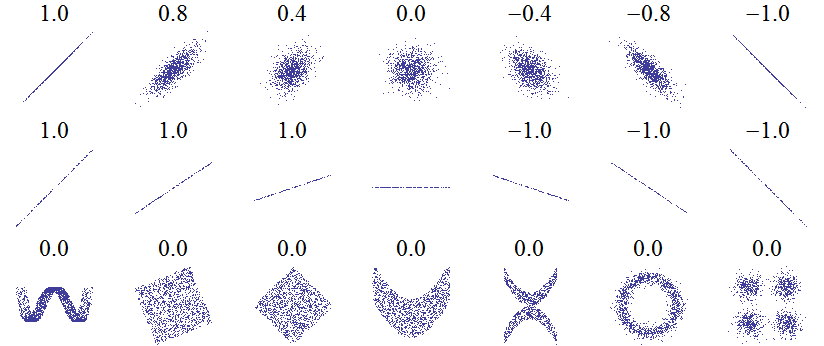
\includegraphics[height=2.5in]{statistics/Correlation_examples.png}}
\caption{Examples of datasets with a range of correlations.}
\label{corr_examples}
\end{figure}

Figure~\ref{corr_examples} is from
\url{http://wikipedia.org/wiki/Correlation_and_dependence}.  It shows
scatterplots and correlation coefficients for several
carefully-constructed datasets.
\index{coefficient!correlation}
\index{scatter plot}
\index{plot!scatter}

The top row shows linear relationships with a range of correlations;
you can use this row to get a sense of what different values of
$\rho$~look like.  The second row shows perfect correlations with a
range of slopes, which demonstrates that correlation is unrelated to
slope (we'll talk about estimating slope soon).  The third row shows
variables that are clearly related, but because the relationship is
non-linear, the correlation coefficient is 0.

The moral of this story is that you should always look at a scatterplot of
your data before blindly computing a correlation coefficient.
\index{correlation coefficient}
\index{coefficient!correlation}

\section{Least squares fit}

Correlation coefficients measure the strength and sign of a
relationship, but not the slope.  There are several ways to estimate
the slope; the most common is a {\bf linear least squares fit}.  A
``linear fit'' is a line intended to model the relationship between
variables.  A ``least squares'' fit is one that minimizes the mean
squared error (MSE) between the line and the data\footnote{See
  \url{http://wikipedia.org/wiki/Simple_linear_regression}.}.
\index{least squares fit}
\index{linear least squares}
\index{coefficient!correlation}
\index{linear regression}

Suppose we have a sequence of points, $Y$, that we want to express as a
function of another sequence $X$.  If there is a linear relationship
between $X$~and $Y$~with intercept $b$~and slope $m$, we
expect each $y_{i}$ to be roughly $m x_i + b$.
\index{residual}

But unless the correlation is perfect, this prediction is only
approximate.  The deviation, or {\bf residual}, is 

\[ \epsilon_{i}~=~(m x_{i}+b)~-~y_{i} \]

The residual might be due to random factors like measurement error,
or non-random factors that are unknown.  For example, if we are
trying to predict weight as a function of height, unknown factors
might include diet, exercise, and body type.
\index{slope}
\index{intercept}

If we get the parameters $b$~and $m$~wrong, the residuals
get bigger, so it makes intuitive sense that the parameters we want
are the ones that minimize the residuals.

As usual, we could minimize the absolute value of the
residuals, or their squares, or their cubes, etc.  The most common
choice is to minimize the sum of squared residuals
%
\[ \min_{m,b} \sum \epsilon_i^2 \]
%
Why?  There are three good reasons and one bad one:

\begin{itemize}

\item Squaring has the obvious feature of treating positive and
negative residuals the same, which is usually what we want.

\item Squaring gives more weight to large residuals, but not
so much weight that the largest residual always dominates.

\item If the residuals are independent of $x$, random, and normally
  distributed with $\mu~=~0$ and constant (but unknown) $\sigma$, then
  the least squares fit is also the maximum likelihood estimator of
  $b$~and $m$.\footnote{See Press et al., {\em Numerical Recipes in C},
    Chapter 15 at \url{http://www.nrbook.com/a/bookcpdf/c15-1.pdf}.}
\index{MLE}
\index{maximum likelihood estimator}

\item The values of $\hat{m}$ and $\hat{b}$ that minimize
  the squared residuals can be computed efficiently.

\end{itemize}

That last reason made sense when computational efficiency was more
important than choosing the method most appropriate to the problem
at hand.  That's no longer the case, so it is worth considering
whether squared residuals are the right thing to minimize.
\index{computation}

For example, if you are using values of $X$~to predict values of $Y$,
guessing too high might be better (or worse) than guessing too low.
In that case you might want to compute some cost function,
cost $(\epsilon_{i})$, and minimize total cost.
\index{cost function}

However, computing a least squares fit is quick, easy and often good
enough, so here's how:

\begin{enumerate}

\item Compute the sample means, $\bar{x}$~and $\bar{y}$, the variance
of $X$, and the covariance of $X$~and $Y$.

\item The estimated slope is
%
\[ \hat{m} = \frac{Cov(X,Y)}{Var(X)} \]
%
\item And the intercept is
%
\[ \hat{b} = \bar{y} - \hat{m} \bar{x} \]
%
\end{enumerate}

To see how this is derived, you can read
\url{http://wikipedia.org/wiki/Numerical_methods_for_linear_least_squares}.




\section{Goodness of fit}
\index{goodness of fit}
\index{fit, goodness}

Having fit a linear model to the data, we might want to know how good
it is.  Well, that depends on what it's for.  One way to evaluate a
model is its predictive power.

In the context of prediction, the quantity we are trying to guess is
called a {\bf dependent variable} and the quantity we are using to
make the guess is called an {\bf explanatory} or {\bf independent
  variable}.
\index{dependent variable}
\index{explanatory variable}
\index{independent variable}
\index{coefficient!determination}

To measure the predictive power of a model, we can compute the {\bf
  coefficient of determination}, more commonly known as ``R-squared'':
%
\[ R^2 = 1 - \frac{Var(\epsilon)}{Var(Y)}\]
%
To understand what $R^2$ means, suppose (again) that you are trying
to guess someone's weight.  If you didn't know anything about them,
your best strategy would be to guess the average weight, $\bar{y}$; in
that case the error of your guesses would be $Var(Y)$:
%
\[\frac{1}{n} \sum (\bar{y} - y_i)^2 = Var(Y) \]
%
But if I told you their height $x_i$, you would guess $\hat{m} x_i + \hat{b} $; in that case your mean standard error (MSE) would be $Var(\epsilon)$.
%
\[ MSE = 
\frac{1}{n} \sum ((\hat{m} x_i + \hat{b}) - y_i)^2 =
Var(\epsilon) \]
%
So the term $Var(\epsilon)/Var(Y)$ is the ratio of mean squared error with
and without the explanatory variable, which is the fraction of
variability left unexplained by the model.  The complement, $R^2$,
is the fraction of variability explained by the model.
\index{variability}

If a model yields $R^2~=~0.64$, you could say that the model explains
64\% of the variability, or it might be more precise to say that it
reduces the MSE of your predictions by 64\%. In the context of a linear least squares model, it turns out that
there is a simple relationship between the coefficient of
determination and Pearson's correlation coefficient, $\rho$:
\[ R^2 = \rho^2  \]

$R^2$ is often refer to as the correlation coefficient.

In practice a calculator or computer is used to calculate the values $m, b$ and $R^2$.  For reference, in EXCEL, the regression coefficients can be found as

\[b={\rm INTERCEPT}\left(Y_{ARRAY},X_{ARRAY}\right)\] 
\[m={\rm SLOPE}(Y_{ARRAY},X_{ARRAY})\] 
\[R^2={\rm RSQ}(Y_{ARRAY},X_{ARRAY})\]
 
It turns out that Excel has a particularly convenient utility for carrying out such calculations: A function called LINEST (which stands for LINE STatistics). To access the uncertainties in the slope and intercept do the following:

Using the mouse, highlight a region of empty cells that is two columns wide by five rows tall. This is where you will be inserting the results from LINEST.
2. Without deselecting the highlighted region, go to the formula bar and type the following "=LINEST(ydata,xdata,true,true)" where "ydata" indicates the cell numbers corresponding to the range of y data (e.g. it might read B2:B10 if you have y data in cells B2, B3,...,B10). The words "true" ought to literally appear as true comma true. Next, instead of hitting "Enter" simultaneously type 
"shift-ctrl-enter". That is, depress and hold down the shift key, the
control key, and finally, the enter key. A $2\times 5$ matrix of numbers should appear in the highlighted cells. The upper left column is the
slope, while the upper right number is the intercept.
The second row holds the uncertainties in those numbers. In particular,
the uncertainty in the slope is the second number down from the top in the left-most column.



\section{Error propagation rules}

\begin{itemize}
\item
The {\em Absolute Error} of a quantity $Z$ is given by $\sigma(Z)$, is equal or larger than zero.
\item
The {\em Relative Error} of a quantity $Z$ is given by $\frac{\sigma(Z)}{|Z|}$, is equal or larger than zero.
\item
To determine the error in a quantity $Z$ that is the {\em sum} of other quantities,
you {\em add the absolute errors} of those quantities (Rules 2,3 below). 
To determine the error in a quantity $Z$ that is the {\em product} of other quantities,
you {\em add the relative errors} of those quantities (Rules 4,5 below).
\end{itemize}

%%\begin{table}[htp]
\begin{center}
\begin{tabular}{c l l}
  & {\bf Relation} &{\bf Error} \\ \hline \\
1. & $Z=cA$         & $\sigma(Z)=|c|\sigma(A)$  \\
2. & $Z=A+B+C+\cdots$ & $\sigma(Z)=\sqrt{(\sigma(A))^2 + (\sigma(B))^2
  +(\sigma(C))^2 + \cdots}$ \\
3. & $Z=A-B-C-\cdots$ & $\sigma(Z)=\sqrt{(\sigma(A))^2 + (\sigma(B))^2
  +(\sigma(C))^2 + \cdots}$   \\
4. & $Z=A \times B \times C \times \cdots$
  & $\frac{\sigma(Z)}{|Z|} = \sqrt{\left(\frac{\sigma(A)}{|A|}\right)^2 + \left(\frac{\sigma(B)}{|B|}\right)^2
  + \left(\frac{\sigma(C)}{|C|}\right)^2 + \cdots}$ \\
5. & $Z=\frac{A}{B}$ & $\frac{\sigma(Z)}{|Z|}
  =\sqrt{\left(\frac{\sigma(A)}{|A|}\right)^2+\left(\frac{\sigma(B)}{|B|}\right)^2}$ \\
6. & $Z=A^{b}$      & $\frac{\sigma(Z)}{|Z|}
  =\sqrt{\left(|b|~\frac{\sigma(A)}{|A|}\right)^2}$  \\
\end{tabular}
\end{center}
%%\label{table:errorrules}
%%\end{table}
Note that in the table, error terms are {\em always\/} added even when the relation is a subtraction.
\begin{itemize}
%%\vspace{-15mm}
\addtolength{\itemsep}{-0.5\baselineskip}
\item
$a, b, c, \ldots, z$ represent constants
\item
$A, B, C, \ldots, Z$ represent measured or calculated quantities
\item
$\sigma(A), \sigma(B), \sigma(C), \ldots, \sigma(Z)$ represent the errors in
$A, B, C, \ldots, Z$, respectively.
\end{itemize}

\section*{How to derive an error equation}
Let's use the change of variable method to determine the error equation for the
following expression: 

\begin{equation}
  y = \frac{M}{m}\sqrt{~0.5~kx} \\
  \label{eq:original}
\end{equation}

\begin{itemize}
\item
Begin by rewriting Equation~\ref{eq:original} as a product of terms:
\end{itemize}
\begin{eqnarray}
  y & = & M~*~m^{-1}~*~ \left[~0.5~*~k~*~x~*\right]~^{1/2} \\ 
    & = & M~*~m^{-1}~*~0.5^{1/2}~*~k^{1/2}~*~x^{1/2}~ 
  \label{eq:productofterms}
\end{eqnarray}

\begin{itemize}
\item
Assign to each term in Equation~\ref{eq:productofterms} a new variable name 
$A,B,C,\dots$~, then express $v$ in terms of these new variables, 
\end{itemize}
\begin{equation}
  y = A~*~B~*~C~*~D~*~E
\label{eq:product}
\end{equation}

\begin{itemize}
\item
With $\sigma(y)$ representing the error or uncertainty in the magnitude of $y$,
the error expression for $y$ is easily obtained by applying Rule 4 to the 
product of terms Equation~\ref{eq:product}: 
\end{itemize}

\begin{equation}
  \frac{\sigma(y)}{|y|} = \sqrt{ \left(\frac{\sigma(A)}{|A|}\right)^2~+~\left(\frac{\sigma(B)}{|B|}\right)^2~+~
  \left(\frac{\sigma(C)}{|C|}\right)^2~+~\left(\frac{\sigma(D)}{|D|}\right)^2~+~\left(\frac{\sigma(E)}{|E|}\right)^2}
  \label{eq:productoferrors}
\end{equation}

\begin{itemize}
\item
Select from the table of error rules an appropriate error expression 
for each of these new variables as shown below. Note that $F$ requires further
simplification since there are two terms under the square root, so we equate these
to a variable $G$: 
\end{itemize}
\begin{center}
\begin{tabular}{lll}
 $A = M$, & $\sigma(A) = \sigma(M)$ & \mbox{Rule 1} \\ 
 $B = m^{-1}$, & $\frac{\sigma(B)}{|B|} 
    = |-1|~\frac{\sigma(m)}{|m|} = \frac{\sigma(m)}{|m|}$ & \mbox{Rule 6} \\
 $C = 0.5^{1/2}$, & $\frac{\sigma(C)}{|C|} 
    = \left|\frac{1}{2}\right|~\frac{\sigma(0.5)}{|0.5|} 
    = 0$ & \mbox{since $\sigma(0.5)=0$} \\ 
 $D = k^{1/2}$, & $\frac{\sigma(D)}{|D|} 
    = \left|\frac{1}{2}\right|~\frac{\sigma(k)}{|k|} = \frac{\sigma(k)}{2|k|}$ 
      & \mbox{Rule 6}\\
 $E = x^{1/2}$, & $\frac{\sigma(E)}{|E|} 
    = \left|\frac{1}{2}\right|~\frac{\sigma(x)}{|x|} 
    = \frac{\sigma(x)}{2|x|}$ & \mbox{Rule 6} \\
\end{tabular}
\end{center}

\begin{itemize}
\item
Finally, replace the error terms into the original error 
Equation~\ref{eq:productoferrors}, simplify and solve for $\sigma(y)$ 
by multiplying both sides of the equation with $y$:
\end{itemize}

\begin{equation}
  \sigma(y) = |y|\sqrt{\left(\frac{\sigma(M)}{|M|}\right)^2 + \left(\frac{\sigma(m)}{|m|}\right)^2 + 
  \left(\frac{\sigma(k)}{2|k|}\right)^2 + \left(\frac{\sigma(x)}{2|x|}\right)^2} 
\end{equation}







%\end{document}



